%%%%Copyright (C) 2024 -  LABORATÓRIO DE APRENDIZADO DE MÁQUINA APLICADO À INDÚSTRIA - https://www.lamia-edu.com/
%%%%UTFPR Campus Santa Helena
%%%%adapted version - SEI-SICITE 2021 UTFPR-GP 
%% This work may be distributed and/or modified under the conditions of the
%% LaTeX Project Public License, either version 1.3 of this license or (at your
%% option) any later version.
%% The latest version of this license is in
%%   http://www.latex-project.org/lppl.txt
%% and version 1.3 or later is part of all distributions of LaTeX version
%% 2005/12/01 or later.
%%
%% This work has the LPPL maintenance status `maintained'.
%%
%% The Current Maintainer of this work is Luiz E. M. Lima.
%%
%% This work consists of the files utfpr-article.sty and utfpr-article.tex.
%%
%% A brief description of this work is in readme.txt.

%% Detecção e aviso sobre comandos obsoletos
% \RequirePackage[l2tabu, orthodox]{nag}

%% Passagem de opções para pacotes
\PassOptionsToPackage{english, main = brazilian}{babel}%% Multilíngue
\PassOptionsToPackage{hyperfootnotes = false}{hyperref}%% Hipertexto extendido

%% Classe de documento e opções
\documentclass[%% Opções: [*] comente para remover; [>] passada para pacotes
  article,%% Tipo de documento: article, book, report, etc. [>]
  a4paper,%% Tamanho de papel: a4paper, letterpaper, etc. [>]
  12pt,%% Tamanho de fonte: 10pt, 11pt, 12pt, etc. [>]
  fleqn,%% Alinhamento de equações à esquerda (comente para centralizado) [>]
  oneside,%% Impressão: oneside (anverso) ou twoside (anverso e verso) [>]
  % twocolumn,%% Texto em duas colunas (comente para uma coluna) [>]
  chapter = TITLE,%% Títulos de capítulos em maiúsculas [*]
  section = TITLE,%% Títulos de seções (secundárias) em maiúsculas [*]
]{abntex2} 

%% Pacotes utilizados
\usepackage[%% Opções
  BibURLs = false,%% Links de URLs nas referências: true ou false
  ABNTNum = none,%% Estilo numérico ABNT: none (AUTOR, ANO), dflt (1) e brkt [1]
]{utfpr-article}

\thanksmarkseries{arabic}

\usepackage{booktabs}
\usepackage{multirow}
\usepackage{float}
\usepackage{lipsum}
\usepackage{changepage}
\usepackage{setspace}

\usepackage{background}
\backgroundsetup{contents={
\includegraphics[scale=0.9]{Logos/sicite_banner.pdf}},
	scale=1,placement=top,opacity=1,position={7.96cm,2.6cm}} 

%% Quadros
%---------------------------------
%Numbered environment
\newcounter{quadro}[section]
\newenvironment{quadro}[1][]{\refstepcounter{quadro}\par\smallskip
   \noindent \footnotesize{\textbf{Quadro~\thequadro #1 -- } \rmfamily}{\smallskip}}

%% Arquivo de referências
\addbibresource{utfpr-article.bib}

%% Informações do documento
%%%% Título
\titulo{%
TITULO (LETRA MAIÚSCULA, NEGRITO, FONTE TIMES NEW ROMAN, TAMANHO  12; CENTRALIZADO)
}

\renewcommand{\thefootnote}{\arabic{footnote}}


%%%% Autor(es) e afiliação(ões)
\autor{%
Nome completo do Bolsista/Voluntário
  \thanks{%
    \affil{Coordenação de Ciência de Computação}% 
    \sep\email{bolsia@alunos.utfpr.edu.br}%
    %\sep\orcid{0000-0000-0000-0000}% Excluir linha caso ORCID seja inexistente
  }%
 \and Nome completo do Orientador%
  \thanks{%
    \affil{Coordenação de Ciência de Computação}%
    \sep\email{orientador@utfpr.edu.br}%
    %\sep\orcid{0000-0000-0000-0000}%% Excluir linha caso ORCID seja inexistente
  }%
  \\
  \and Nome completo do Coautor(es)%
  \thanks{%
    \affil{Coordenação de Ciência de Computação}%
    \sep\email{coautor(es)@utfpr.edu.br}%
    %\sep\orcid{0000-0000-0000-0000}
  }%
}



%%%% Câmpus: {SIGLA}; {NOME}
\campus{SH}{Câmpus Santa Helena}
%%%% Departamento, coordenação, programa ou curso: [LOGO]; {SIGLA}; {NOME}
\departamento[depto]{DEPTO}{COCIC}
%%%% Local: {CIDADE, ESTADO, PAÍS}
\local{Santa Helena, Paraná, Brasil}
%%%% Data: comente para gerar a data atual
\data{}

%% Ferramenta para criação de índices
\makeindex%

%%Espaçamento duplo
\usepackage{leading}
%% Início do documento
\begin{document}

%\pretextual%% Elementos pré-textuais

\begin{paginadetitulo}%% Página de título

\begin{ambienteresumo}%% Resumo
\leading{12pt}
Formatação do texto: Fonte Times New Roman, tamanho 12, alinhamento justificado e espaçamento simples. Deverá ser escrito em português, com extensão de 4 a 6 páginas em tamanho A4, com margem superior de 4cm e inferior 2,5 cm; esquerda e direita de 3,0 cm. O Resumo do trabalho deve conter entre 1500 e 2500 caracteres com os espaços. Deve ter introdução, objetivo, metodologia, resultados e considerações finais.

\palavraschave{1 palavra-chave.\ 2 palavra-chave.\ 3 palavra-chave.}%% Palavras-chave
\end{ambienteresumo}
\end{paginadetitulo}
\textual%% Elementos textuais

\leading{18pt}
\section{INTRODUÇÃO}\label{sec:intro}

\begin{flushleft}%Deixar primeiro parágrafo alinhado a esquerda
A seção de Introdução deve contextualizar a ação, apresentando a justificativa do trabalho de forma clara, a revisão de literatura e no final o(s) objetivo(s). O texto deverá ser digitado em Fonte Times New Roman, tamanho 12, justificado, espaçamento entre linhas de 1,5.
\end{flushleft}

\begin{citacao}
\normalsize
    As citações diretas que ultrapassarem três (3) linhas deverão ser escritas na mesma fonte do texto, porém com tamanho reduzido 11(onze), com recuo de quatro (4) cm da margem, espaçamento simples e sem aspas.
\end{citacao}

Quando for referenciar outros trabalhos utilize \cite{gonccalves2002} ou \textcite{gonccalves2002}.

\section{METODOLOGIA}

\begin{flushleft}%Deixar primeiro parágrafo alinhado a esquerda
A seção de Metodologia deve ser concisa, mas suficientemente clara, de modo que o leitor entenda e possa reproduzir os procedimentos utilizados, apresentando as características do público, o(s) instrumento(s) de coleta e os procedimentos utilizados.
\end{flushleft}

\subsection{Subseção}

\begin{flushleft}%Deixar primeiro parágrafo alinhado a esquerda
As seções deverão ser escritas em todas as letras maiúsculas e em negrito e as subseções apenas com a primeira letra maiúscula e em negrito, alinhadas à esquerda e enumeradas. Não deverão ser utilizados: ponto, hífen, travessão ou qualquer outro sinal após o indicativo numérico da seção e subseção. As grandezas deverão ser expressas no Sistema Internacional (SI), e a terminologia científica (incluindo a nomenclatura e os símbolos gregos) deverá seguir as convenções internacionais de cada área em questão.
\end{flushleft}

O primeiro parágrafo de cada seção ou subseção deve estar alinhado à margem esquerda. Os demais parágrafos redigidos com deslocamento de 1,25cm na primeira linha.

\section{RESULTADOS E DISCUSSÃO}

\begin{flushleft}%Deixar primeiro parágrafo alinhado a esquerda
Neste item devem ser apresentados e discutidos os resultados mensuráveis e qualitativos da ação de extensão. Poderão ser inseridas tabelas, figuras e gráficos, em conformidade com as normas vigentes da ABNT. As grandezas deverão ser expressas no Sistema Internacional (SI), e a terminologia científica (incluindo a nomenclatura e os símbolos gregos) deverá seguir as convenções internacionais de cada área em questão.
\end{flushleft}

As tabelas precisam conter título e numeração sequencial, conforme o modelo da Tabela \ref{tab:areas}, com fonte \textit{Times New Roman} tamanho 12 para título e conteúdo e tamanho 10 para notas (quando necessário).

\begin{table}[ht]
\centering
\caption{Modelo}
\begin{tabular}{@{}ccccc@{}}
\toprule
\textbf{ÁREAS}                 & \textbf{UN} & \textbf{Pot} & \textbf{SP} & \textbf{TOTAL} \\ \midrule
Interdisciplinar      & 2  & 2   & 2  & 6     \\
Biológicas e da Saúde & 2  & 2   & 2  & 6     \\
Exatas e Tecnológicas & 2  & 2   & 2  & 6     \\
Humanas e Artes       & 2  & 2   & 2  & 6     \\ \midrule
TOTAL                 & 8  & 8   & 8  & 24    \\ \bottomrule
\end{tabular}
\newline \footnotesize	 Fonte: Modelo
\label{tab:areas}
\end{table}

As figuras precisam ser de boa qualidade e nítidas. Também devem ser nomeadas e numeradas, com fonte Times New Roman tamanho 10, seguindo o modelo da Figura \ref{fig:consumos}.

\captionsetup[figure]{width=0.75\textwidth}
\begin{figure}[h]
\centering%
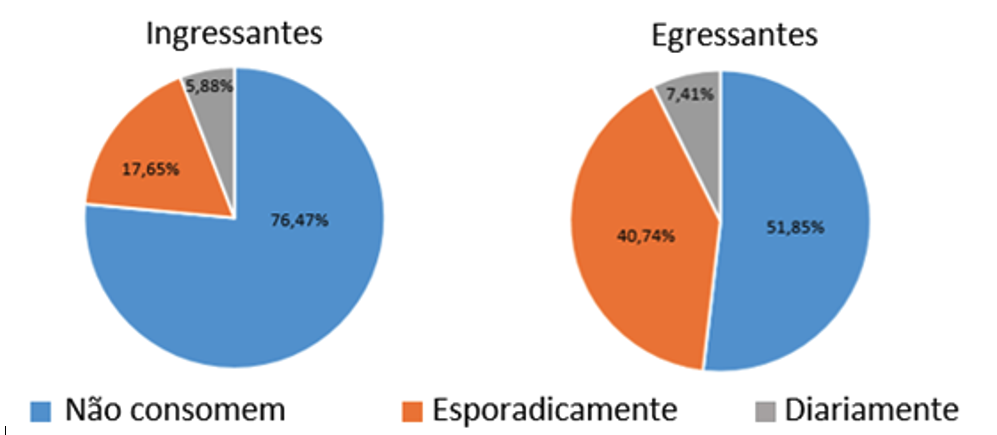
\includegraphics[width = 0.75\columnwidth]{./Figuras/imagem_consumo}
\caption{Consumo semanal de feijão entre estudantes ingressantes na Universidade, Câmpus Universitário. Dados representados em porcentagem ingressantes (N=34) e Egressantes (N=27). Fonte: Modelo.}
\label{fig:consumos}
\end{figure}


\section{CONSIDERAÇÕES FINAIS}

\begin{flushleft}%Deixar primeiro parágrafo alinhado a esquerda
Apontar as considerações finais da pesquisa ou extensão.
\end{flushleft}


\postextual%% Elementos pós-textuais

\section*{Agradecimentos}

Agradecer à agência de fomento CNPq, Fundação Araucária, UTFPR, ou outra.


\section*{REFERÊNCIAS}
\leading{13.8pt}
\printbibliography[heading=none]%% Referências

%% Fim do documento
\end{document}
